\section{Struktur Organisasi}
\label{sec:struktur}

\begin{figure}[ht!]
    \centering
    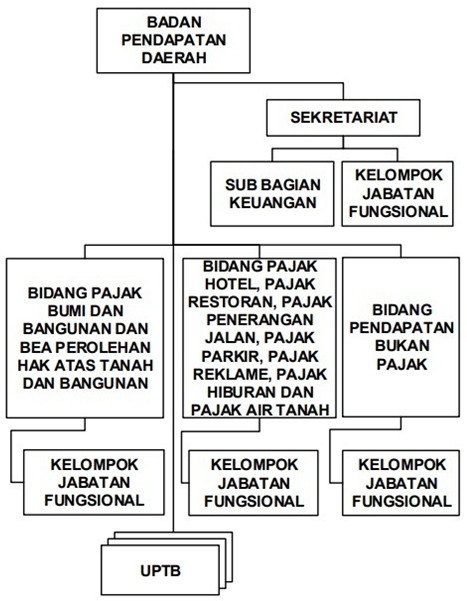
\includegraphics[width=0.54\textwidth]{gambar/struktur-organisasi.png}
    \caption{Struktur Organisasi Bapenda Kota Surabaya}
    \label{fig:struktur-organisasi}
\end{figure}

Berdasarkan struktur organisasi resmi, Badan Pendapatan Daerah (Bapenda) Kota Surabaya dipimpin oleh seorang Kepala Badan. Secara garis besar, struktur ini terbagi menjadi dua komponen utama: unsur pendukung administratif yang direpresentasikan oleh Sekretariat, dan unsur pelaksana teknis yang terdiri dari tiga Bidang utama serta Unit Pelaksana Teknis Badan (UPTB).

Berikut adalah penjelasan rinci mengenai tugas dan fungsi dari setiap unit dalam struktur organisasi Bapenda Kota Surabaya:
\begin{itemize}
    \item Struktur Utama \\
    Struktur utama Bapenda terdiri dari unit-unit yang berfungsi sebagai pendukung jalannya administrasi dan operasional internal organisasi. Unit-unit ini adalah:
    \begin{enumerate}
        \item Badan Pendapatan Daerah: Merupakan unit utama yang memegang tugas pokok untuk mengelola dan mengumpulkan seluruh pendapatan daerah Kota Surabaya.
        \item Sekretariat: Berada langsung di bawah Kepala Badan, Sekretariat memiliki fungsi vital dalam mengurus administrasi umum, kepegawaian, dan mengelola keuangan internal badan.
        \item Sub Bagian Keuangan: Unit ini berada di bawah koordinasi Sekretariat dan memiliki tugas yang lebih spesifik, yaitu secara khusus menangani proses penganggaran serta pembukuan keuangan internal Bapenda.
        \item Kelompok Jabatan Fungsional: Unit ini terdiri dari para pegawai dengan keahlian khusus yang berfungsi untuk mendukung pelaksanaan tugas-tugas teknis organisasi. Seperti yang terlihat pada diagram, Kelompok Jabatan Fungsional ini melekat baik pada Sekretariat maupun pada setiap Bidang Teknis.
    \end{enumerate}
    \item Bidang Teknis dan Pelaksanaan \\
    Bagian ini merupakan unit-unit inti yang melaksanakan fungsi utama Bapenda dalam hal pemungutan pendapatan dari berbagai sektor. Struktur ini terdiri dari tiga bidang utama dan satu unit pelaksana:
    \begin{enumerate}
        \item Bidang PBB dan BPHTB: Bidang ini memiliki fokus teknis untuk mengelola dan memungut pajak yang berkaitan dengan properti dan hak atas tanah. Sesuai dengan yang tertera pada diagram, nama lengkap bidang ini adalah Bidang Pajak Bumi dan Bangunan dan Bea Perolehan Hak atas Tanah.
        \item Bidang Pajak Lainnya: Bidang ini bertanggung jawab mengurus berbagai jenis pajak barang dan jasa di luar PBB dan BPHTB. Rincian tugasnya mencakup pengelolaan Pajak Hotel, Pajak Restoran, Pajak Penerangan Jalan, Pajak Parkir, Pajak Reklame, Pajak Hiburan, dan Pajak Air Tanah.
        \item Bidang Pendapatan Bukan Pajak: Unit teknis ini memiliki tanggung jawab untuk mengelola sumber-sumber pendapatan daerah yang berasal dari luar pajak utama, seperti retribusi daerah dan pendapatan lain-lain di luar pajak.
        \item Unit Pelaksana Teknis Badan (UPTB): Berada di bawah koordinasi dan bertanggung jawab kepada tiga Bidang Teknis, UPTB merupakan unit yang bertugas sebagai pelaksana operasional teknis Bapenda di wilayah-wilayah kerja yang telah ditentukan.
    \end{enumerate}
\end{itemize}